\chapter{Small Sphere Experiment}
\label{chap:SmallSphere}

\textit{The work presented here has been presented as an invited oral presentation by Lindsay MacDonald at AIC 2017 \citep{macdonald_melanopsin_2017}\footnote{The proceedings are not currently available online, though a note at \url{https://aic-color.org/page-18077} suggests that they will soon be available.}.}


\section{Summary}

This experiment was performed to develop upon the Large Sphere experiment (Chapter \ref{chap:LargeSphere}) by narrowing down the number of variables and more directly exploring the question of whether melanopsin plays a role in colour constancy. Observers were adapted to one of two perceptually metameric conditions, one with a high melanopic content and one with a low melanopic content. Statistically significant but low magnitude differences were found between conditions for two out of three observers. For the two observers who performed repeated trials, inter-trial variability was high, and of a similar magnitude to inter-condition differences. One observer provided drastically difference responses during the repeat sessions; hardware issues which may cause such a difference are discounted, and remaining hypotheses for what may have caused such a large distinction are discussed. 

This study was approved by the \gls{UCL} Ethics committee (Project ID Number: 9357/003), application attached as Appendix \ref{app:ethics3}. Code and data are provided: \url{https://github.com/da5nsy/Small-Sphere}.

\section{Introduction}

Several key alterations were made to address limitations of the Large Sphere experiment:

\begin{enumerate}
    \item Instead of 16 surround conditions, only two were included.
    \begin{enumerate}
        \item These two conditions were generated through use of narrow-band \glspl{LED} rather than filtered white light, designed to be perceptual metamers for individual observers, but with maximally different levels of melanopic activation.
    \end{enumerate}
    \item Instead of 16 lightness conditions, only 5 were included. This was done so that more repeated conditions could be measured within the same time-span.
    \item The sphere used was smaller, and the inner surface was painted with a higher reflectance paint, which raised the level of illumination to roughly 10 cd/m$^2$.
\end{enumerate}

Further details on all of the above amendments will be included in the following sections. Three observers were tested (the author and two colleagues of a similar age), with repeats of each condition. The null hypothesis that this experiment aims to test is that melanopsin activation does not alter an observers' perceptual white point.

\section{Materials and Methods}

\subsection{Hardware}

The sphere used in this experiment was 400mm in diameter, with ports of similar functions to those in the Large Sphere. On one side there was a padded port for an observer's face. Mirroring this was a circular aperture of 52mm diameter (giving a viewing angle of roughly 6.6 degrees), through which an LCD screen was visible. At the top of the sphere was a port through which adapting illumination was provided. An additional port, on the observer's side of the base, was added such that the illumination provided to the sphere could be unobtrusively monitored throughout experiments.

\begin{figure}[htbp]
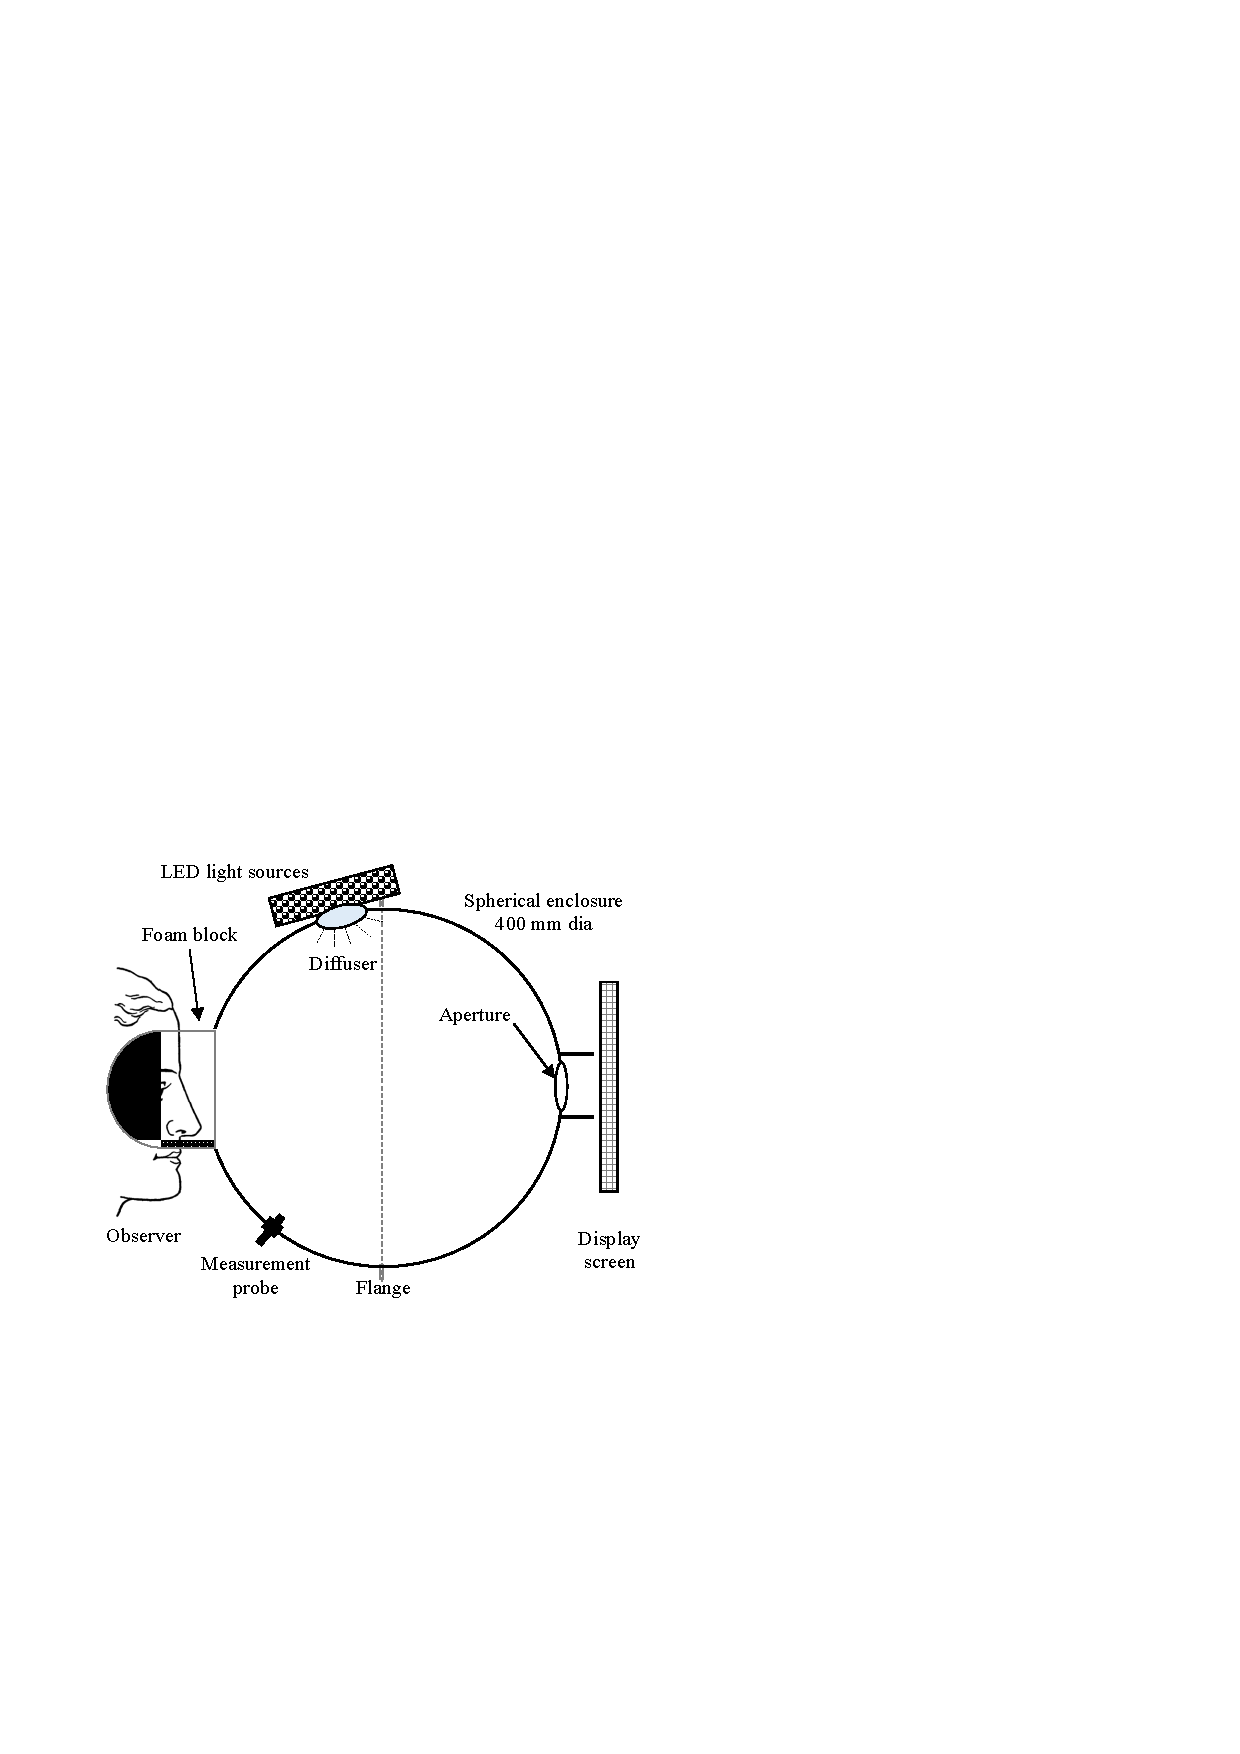
\includegraphics[max width=\textwidth,center]{figs/SmallSphere/diagram.pdf}
\caption{The small sphere set up, reproduced from \citet{macdonald_melanopsin_2017}, courtesy of Lindsay MacDonald.}
\label{fig:diagram}
\end{figure}

\begin{figure}[htbp]
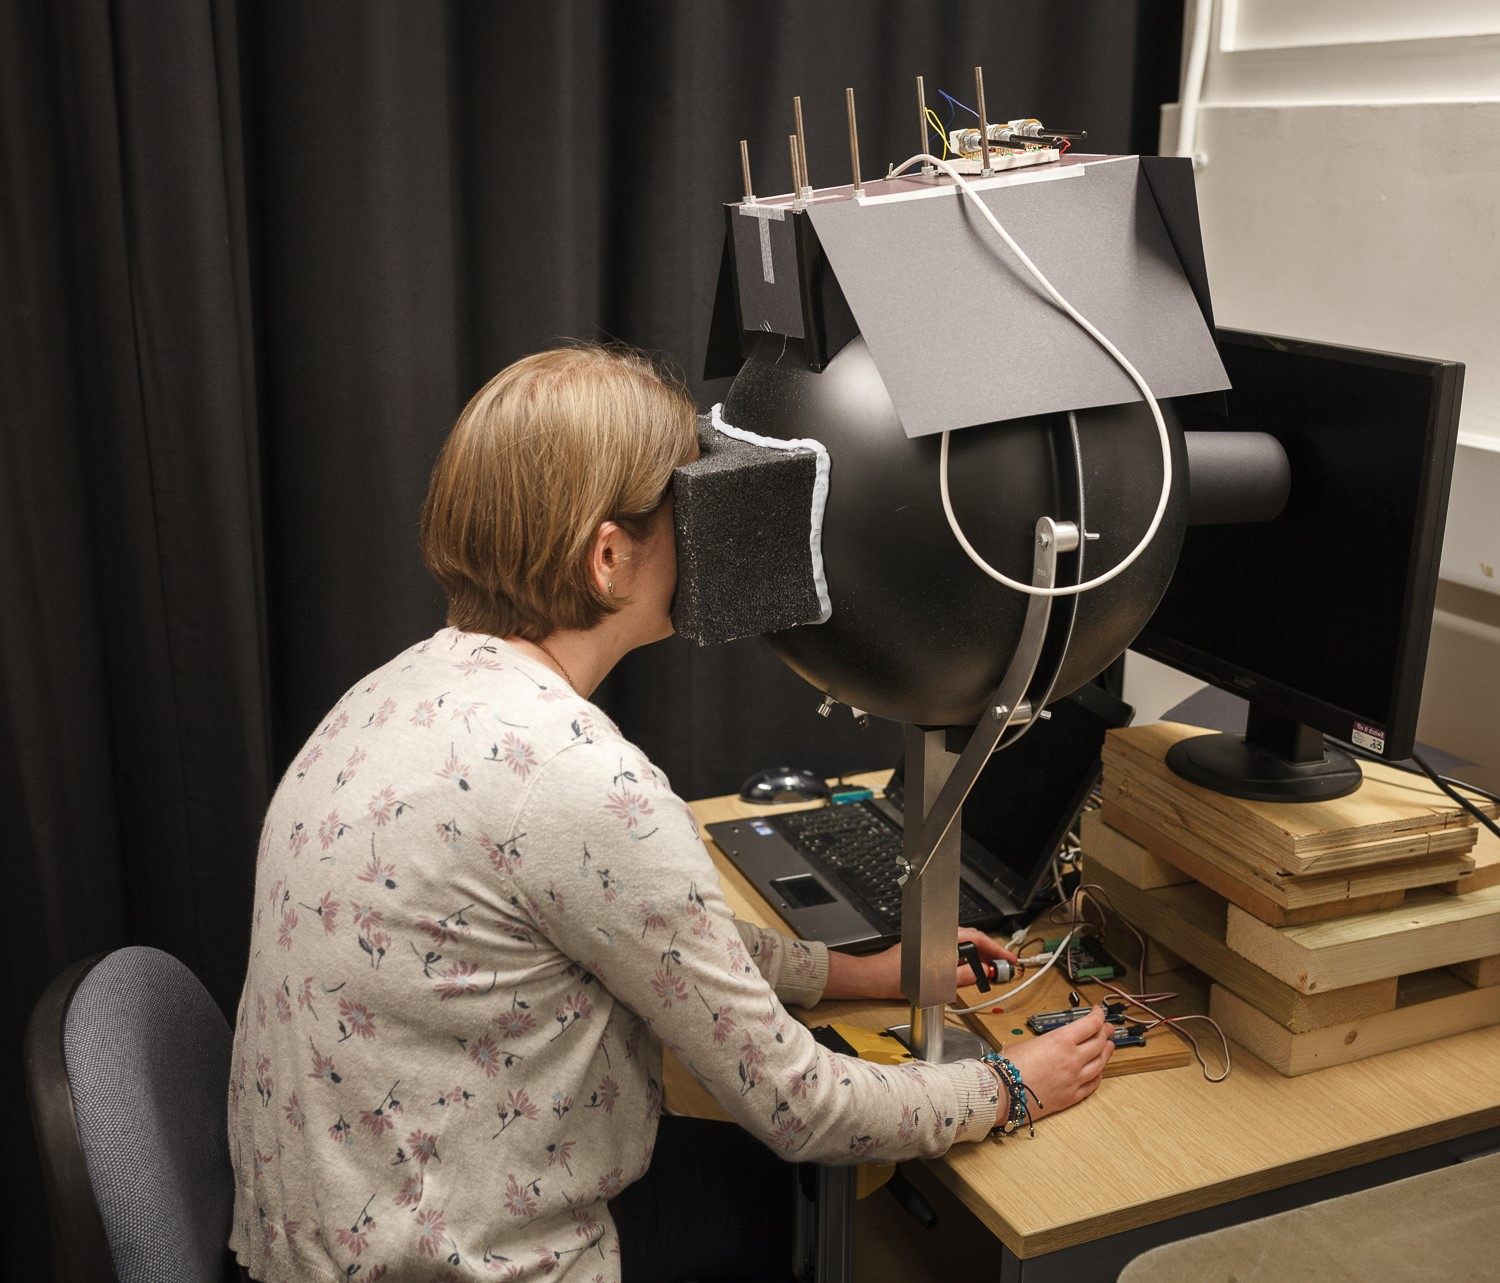
\includegraphics[max width=\textwidth,center]{figs/SmallSphere/SSphoto.jpg}
\caption{An observer sits with two hands on the sliders. Actual experiments were performed with the room lights turned off}
\label{fig:SSphoto}
\end{figure}

\subsection{The Sphere}

The sphere used in this experiment was smaller than that in the previous experiments (hence the experiment short-hand names) and this served several purposes. The illumination in the Large Sphere had been very low, partly such that rod interactions would be made visible, and partly due to practical limitations. The grey paint on the interior of the Large Sphere was chosen to limit specular reflections, but it meant that overall illumination levels were very low. In the small sphere, it was hoped that by reducing the size of the sphere it would be possible to increase the level of illumination, as it would be spread across a smaller surface. Additionally, of practical concern, it was easier to find experimental space for a smaller sphere.

Several paints were trialled for use in the small sphere. The required conditions were that they were available as a spray, and provided as `matt white'. Sample patches were sprayed upon a piece of opaque perspex to assess finish and spectral reflectance. It was seen as beneficial if: the finish had a very fine grain and as little gloss to it as possible, the surface reflectance was high, and the \gls{SRF} was as uniform across the spectrum as possible. It was also considered a requisite requirement that any paint should not include any fluorescent whitening agents (such as can be seen in the `white paper' shown in Figure \ref{fig:spray}).

Measurements of the \glspl{SRF} of the 8 tested spray-paints, and further details of the spray-paints themselves, can be seen in Figure \ref{fig:spray}. Measurements were made with a \gls{PR650}, illuminated at 45$^{\circ}$ and measured at 90$^{\circ}$. It can be seen that Montana Gold Sh. White Cream and Pebble, along with MTN 94 RV-198 are either too low in reflectance or not uniform in spectral reflectance across the spectrum. The two with the most desirable finishes were the Flame Blue and MTN Water Based paints. The MTN Water Based paint was chosen due to its particularly fine-grain finish.

%The sharp drop off in the \glspl{SRF} suggest that most of the tested paints were titanium-based (based on comparisons to measurements made by \citet{cosentino_fors_2014})\footnote{It is unfortunate in some ways that the \glspl{SRF} drop so rapidly around 400nm, as this means that the one of the chosen LEDs with a peak output of around 400nm will lose a great deal of its power in the interaction with the paint. On the other hand - this decreases the risk to the observer of being exposed to exessive amounts of short wavelength radiation.}.  

\begin{figure}[htbp]
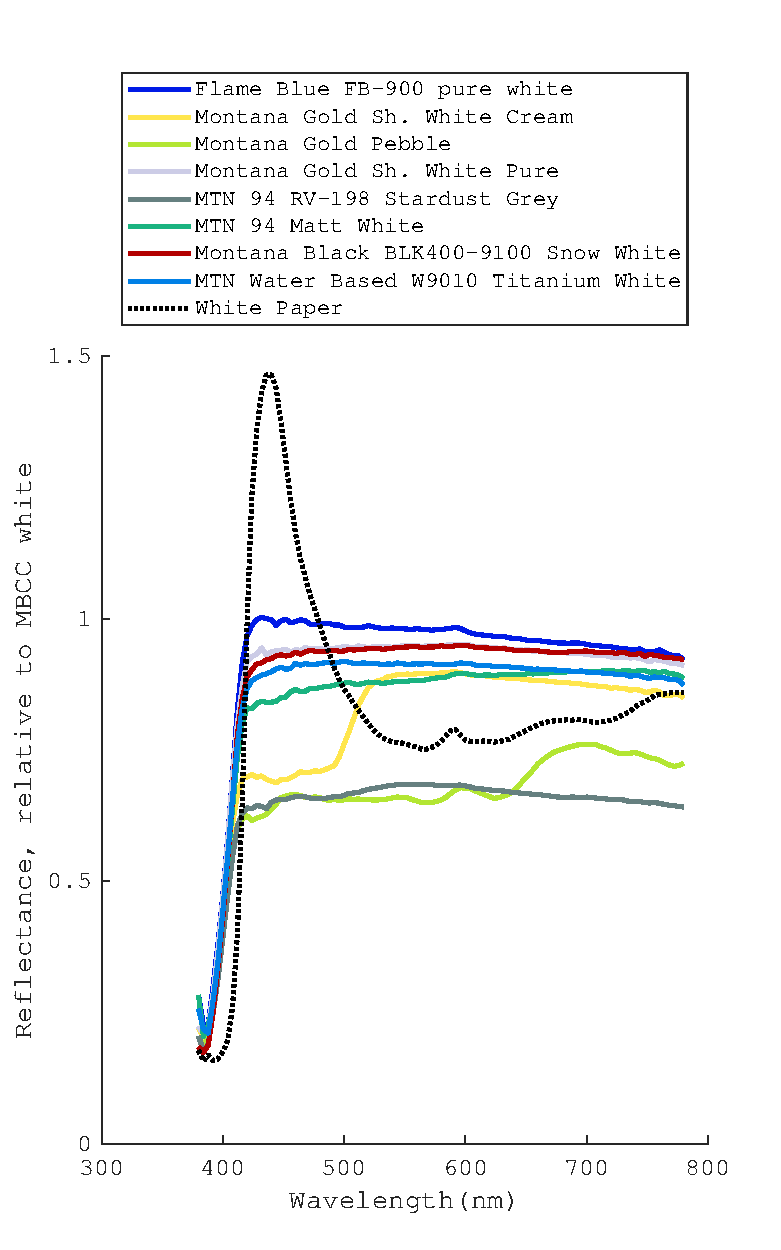
\includegraphics[max width=0.9\textwidth,center]{figs/SmallSphere/VisualiseSPDs_result.pdf}
\caption{The \glspl{SRF} of the 8 tested paints (relative to the white patch of a MacBeth Colour Checker card) with an additional measurement of a piece of white office paper to demonstrate how a fluorescent additive might appear. Data available: \url{https://github.com/da5nsy/Small-Sphere/tree/master/Hardware\%20Specs/WhiteSprayPaints}}
\label{fig:spray}
\end{figure}


\subsection{The Screen}

The screen was offset by roughly 150mm through a short black paper tube in order to limit the interference (either way) between the screen emission and the sphere illumination. 

\subsubsection{Characterisation}

Following issues potentially stemming from uncontrolled variations of display output during the Large Sphere experiment, characterisations of the display output were performed more regularly (after every set of observations), and an additional characterisation protocol was introduced. The adapting illuminant was also monitored throughout every session.

The primary characterisation protocol was as standard - a spectral measurement of the display primaries followed by a ramping through intensity for each display channel from zero output to maximum output\footnote{Controlled by the script available at \url{https://github.com/da5nsy/Small-Sphere/blob/5c6af38c5036a4c0a328a9854427ae8e851e84fd/Hardware\%20Specs/PR650\%20Screen\%20Measurements/PR650displaycharacterisation_DG.m}}. This was only measured for the small portion of the screen which would be seen during experiments.

The secondary characterisation protocol attempted to detect any issues which may arise due to the specific way in which screen output was specified and recorded during the experiment. The main MATLAB experimental script was modified to provide a `characterisation mode', with a greatly reduced number of trials (15 total). This mode otherwise performed in exactly the same way that the main experimental script normally would, and the observer was replaced by the \gls{PR650}, and no effort was made to select neutral points, with a measurement being made of each presentation directly. In this way, a random selection of points were recorded, and through comparison with the recorded `responses', it could be seen whether there was any discrepancy between the expected and actual display output.

\subsection{The LED Rig}

The lighting in this experiment was designed such that two lighting conditions could be defined for each observer which were perceptual metamers (in the periphery, at high temporal frequencies), but which differed in melanopic activation.

Four types of \gls{LED}, to operate as two pairs, were chosen to maximise melanopic contrast between the pairs. An additional limitation was that no LED with a peak wavelength shorter than 400nm was to be used (due to safety concerns).

50 LEDs, mounted in a breadboard, were controlled by an Arduini Uno. %photo?

\begin{itemize}
    \item 20: Bivar UV5TZ-400-15 (henceforth `UV')
    \item 10: Cree C503B-BCS-CV0Z0461 (henceforth `blue')
    \item 10: Cree C503B-AAS-CA0C0251-015 (henceforth `amber')
    \item 10: Cree C503B-RAS-CY0B0AA2 (henceforth `red')
\end{itemize}

%UNOPENED 
%810-6705 C503D-WAN-CCbEb151
%810-6636 C503B-AAN-CY0B0251
%810-0492 C503B-BCN-CV0Z0461

\begin{figure}[htbp]
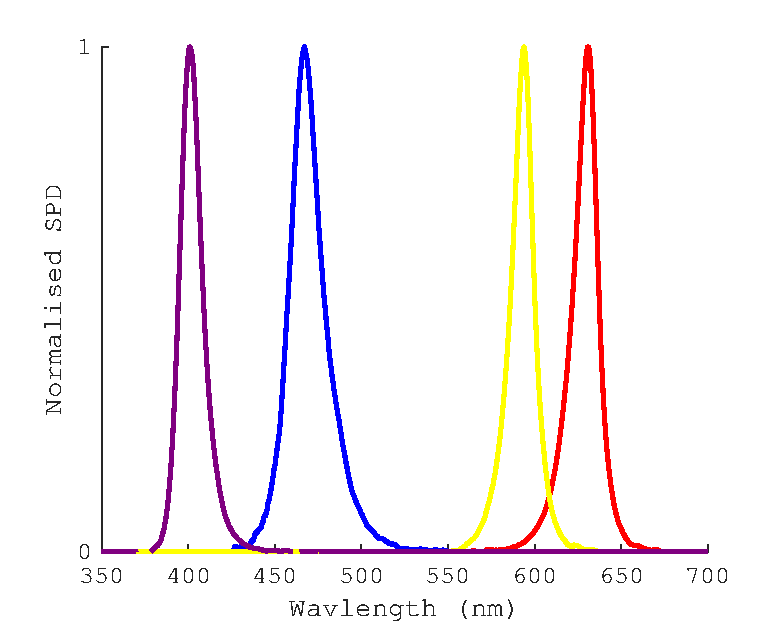
\includegraphics[max width=\textwidth,center]{figs/SmallSphere/LED_SPDs.pdf}
\caption{The normalised \glspl{SPD} of the Small Sphere \glspl{LED}.}
\label{fig:LED_SPDs}
\end{figure}

The arduino script set the \glspl{LED}, via pulse width modulation, to the output levels decided in the perceptual nulling segment of the experiment. The two modes had either the combination of UV and amber, or blue and red, allowing for the chromaticities falling upon the lines shown in Figure \ref{fig:LED_SPDs}. The combinations UV and blue, or amber and red, were never used.

\begin{figure}[htbp]
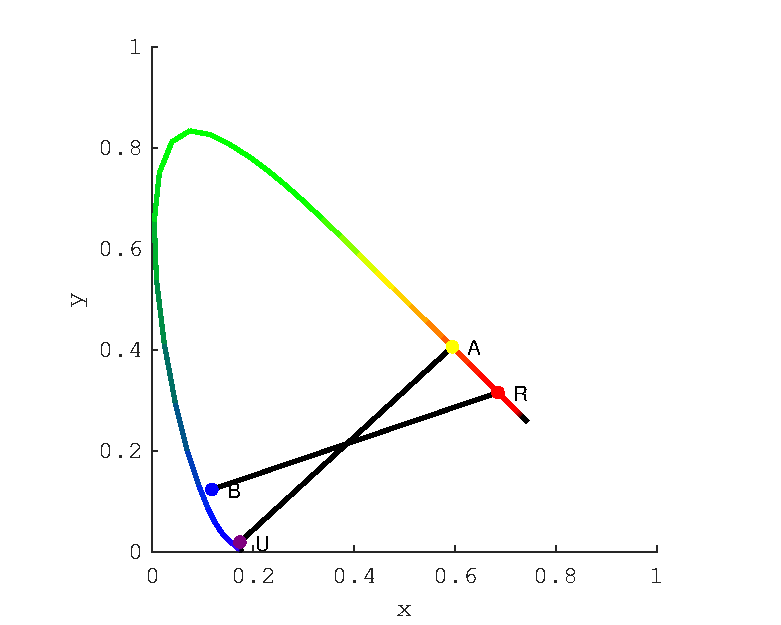
\includegraphics[max width=\textwidth,center]{figs/SmallSphere/LED_cross.pdf}
\caption{The chromaticities of the Small Sphere \glspl{LED} in CIE 1931 space, with lines connecting the pairs which were activated simultaneously. From each pair, illumination with chromaticity values extending along each line was generatable. Even if there were differences in the spectral sensitivities of the observers (compared to the CIE 1931 observer), with these narrow-band primaries there should theoretically always be a point at which the two lines cross.}
\label{fig:LED_cross}
\end{figure}

This breadboard was mounted stably atop the sphere with a perspex diffusion sheet between it and the opening into the sphere. Black card was used to mask stray light, mainly to address the specific concern that light may fall onto the LCD display.

%LM: photo of the construction of the lighting rig (close up)

Throughout the experiments the illumination inside the sphere was measured with an Ocean Optics USB 2000+ through an optical fibre probe mounted to the base of the sphere and directed at a point on the roof of the sphere, opposite the observer. It was expected that the output of the \glspl{LED} may change slightly over time. %fig x?

The melanopic contrast between conditions, in terms of Weber contrast, was 365\%, 309\%, and 488\% for observers DG, HC and LW respectively. The variability in these figures between observers is due to the unique settings that each observer made, described in Section \ref{sec:null}.

\subsubsection{Light safety}
Since illumination of wavelengths shorter than 400nm would be present, it was deemed appropriate to take extra precautions to ensure the safety of participants. 
The implementation of the `BS EN ISO 15004-2:2007 Ophthalmic instruments - Fundamental requirements and test methods - Part 2: Light hazard protection' \citep{iso/tc_172/sc_7_ophthalmic_optics_and_instruments_bs_2007} provided in the Silent Substitution toolbox\footnote{\url{https://github.com/spitschan/SilentSubstitutionToolbox}} created by \citet{spitschan_selective_2015} was used to evaluate the safety of the experimental set-up, and under the default assumptions for pupil size, and with the maximum output from the LEDs, the stimulus was found to be considerably below the limits for type 1 continuous wave instruments. See Appendix \ref{app:ethics3} for further details.

% safety
% The controllers 
% The code
% Characterisation / ongoing measurement

\subsection{Observer Task}

In this experiment there were two stages to the observer task; the first (perceptual nulling) where observers would set the two surround conditions such that they were minimally distinguishable for them, and the second which was an achromatic selection task (much like that performed in the Large Sphere experiment).

\subsubsection{Perceptual Nulling of Peripheral Adapting Field} \label{sec:null}

The basic logic of this experiment is as follows: under the null hypothesis two adapting fields of identical appearance should cause an observer to be adapted in exactly the same way. In order to design two adapting field illuminants which appear identical (perceptual metamers) we can either make predictions based upon standard observers (with parameters set to match our real observers regards age and pupil dilation etc.) or we can employ a process whereby individual observers make minor alterations to two conditions (that are designed such that they could be metamers) until they appear identical. We have opted to use colorimetry as a starting point to choose LED primaries (Figure \ref{fig:LED_cross}), and then allow observers to fine-tune this matching.

We run the risk of falling into circularity here: we ask observers to set two fields such that they appear identical, and then (in a roundabout way) we ask them whether there is any visual difference between them. If melanopsin does have a direct impact upon visual perception we are at risk of accounting for this at this stage. In an attempt to avoid this problem, we perform the perceptual nulling under conditions which we predict should not allow for \gls{ipRGC} involvement, or should minimise such. It seems to be the case that \glspl{ipRGC} do not react strongly over very short timescales ($<$0.5hz \citep{spitschan_human_2017-1}), with cones being much more active in this temporal window, so we chose to alternate rapidly between the two conditions and ask observers to make alterations until there is a minimal visible flicker.

Observers were instructed to fixate upon a small fixation point displayed at the centre of the otherwise dark display. They placed their hands upon three dials which could be independently varied to change the peripheral adapting illumination inside the sphere.

Two modes were presented to observers; one where the two conditions were alternated at 30hz for 1 second followed by a 10 second break, and one where the conditions were alternated at 4hz for 500ms followed by a 1 second break. 

In the first mode the observer was requested only to alter the setting of the first dial, which would change the overall level of the red/blue combination (whilst the uv/amber combination remained at the same level). This was referred to as brightness matching.

During the second mode the observer was requested only to alter the settings of the second and third dials. The second dial would alter the relative contributions of red vs. blue to red/blue condition. The third dial would alter the relative contributions of uv vs. amber to the uv/amber condition. These options can be thought of as traversing the straight lines in Figure \ref{fig:LED_cross}. This was referred to as colour matching.

%LM: photo of observer looking into sphere

The observer was allowed to switch back and forth between these two modes until they were happy with the match. Once an observer had indicated a match, the LED drive values were recorded and these were used for the observer in future sessions.

Observers found this task rather arduous, predominantly due to the inherent difficulty in making colour matches in the periphery. An additional difficulty was that since eye movements were not strictly controlled, if an observer were to look away briefly from the fixation they would be able to see the adapting field with their foveal vision. This was problematic since in most cases the peripheral matches induced strong contrast for foveal perception. Though it was unintentional, this seems to be a particularly effective way of generating the perception of a Maxwell spot \citep{isobe_functional_1955}. Further to this, the authors' experience was that the visible periphery could be further divided, by eccentricity, into two or possibly three areas where a match in one area would not provide a match in both areas.

Despite these difficulties, observers generally found settings which for them resulted in a metameric match (where they could no longer perceive flicker, or perceived very little flicker). 

One observer who initially agreed to take part in this study withdrew at this stage, partly due to a difficulty completing this task, but mainly due to a claustrophobic reaction. Another potential observer withdrew at this stage, since he was unable to make a match using this set of primaries, which we tentatively attribute to incipient cataracts.

This method has since been further developed by \citet{allen_form_2019} who used a 2AFC task instead of a method of manual adjustment to pinpoint areas of perceptual metamerism.

% Observers were...
% Initial metamer setting
\subsubsection{Achromatic Selections}

3 observers took part in the main experiment (the author (DG), HC, and LW). 

The task was identical to that performed in the Large Sphere experiment; using two sliders (controlling the yellow/blue component and the red/green component) to set the foveal stimulus to appear achromatic. The instruction was given to set the central disc such that it appeared not red, green, blue or yellow. As previously noted, instead of 10 runs of L* 85 descending in 5* increments to L* 10, there were 30 runs of a pseudo-randomly permuted (each run) set of stimuli specified such that there was one at every 10 L* interval between 30 L* and 70 L*. The range was reduced so as to minimise the impact of gamut-boundary issues. The L* interval was increased to allow for a greater number of repetitions of specific values within a similar time frame. The order was pseudo-randomly permuted to avoid any trend based effects.

Two observers (HC and LW) performed 4 complete runs each, 2 under each condition. The author completed 2 runs, one under each condition. Each observer only completed one run per day. There was a gap of roughly three months between the initial runs of HC and LW and the repeat runs.

\subsubsection{Data Analysis}

Following calibration, for each observer under each condition, the means and standard deviation were computed for each dimension of CIELAB. 

The data were submitted to a two-dimensional two-sample Kolmogorov-Smirnov test\footnote{Using the function available from \url{https://uk.mathworks.com/matlabcentral/fileexchange/38617-kstest_2s_2d-x1-x2-alpha}.} to compare the two distinct conditions for each observer (including data for repeats where performed). To provide a baseline-check, the same test was applied to the repeated data for like conditions, with the assumption that this would not return a significant difference.

These results were considered alongside measurements of LEDs taken during the experiments.

\section{Results}

\subsection{Primary Data}

A summary of results, where each run is represented by a standard deviation ellipse, is shown in Figure \ref{fig:SSsummary}. This data is summarised numerically in Table \ref{tab:SS}.
%
\begin{figure}[htbp]
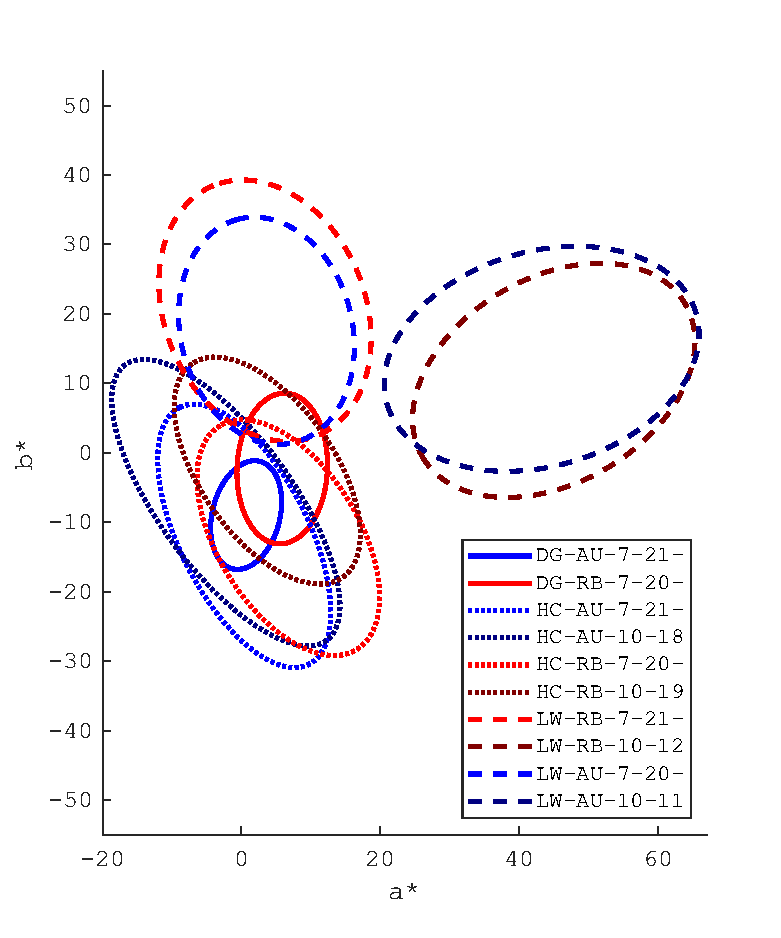
\includegraphics[max width=1.2\textwidth,center]{figs/SmallSphere/SSsummary.pdf}
\caption{A summary of all primary data in CIELAB. Ellipses represent 1 standard deviation in the primary and orthogonal axes. The legend lists observer (`DG' / `HC' / `LW'), followed by condition (`AU' - amber / UV, `RB' - red / blue) and date in M:D format.}
\label{fig:SSsummary}
\end{figure}
%
Break downs for each observer, showing each achromatic setting are shown in Figures \ref{fig:SS_DG} - \ref{fig:SS_LW}.

\begin{figure}[htbp]
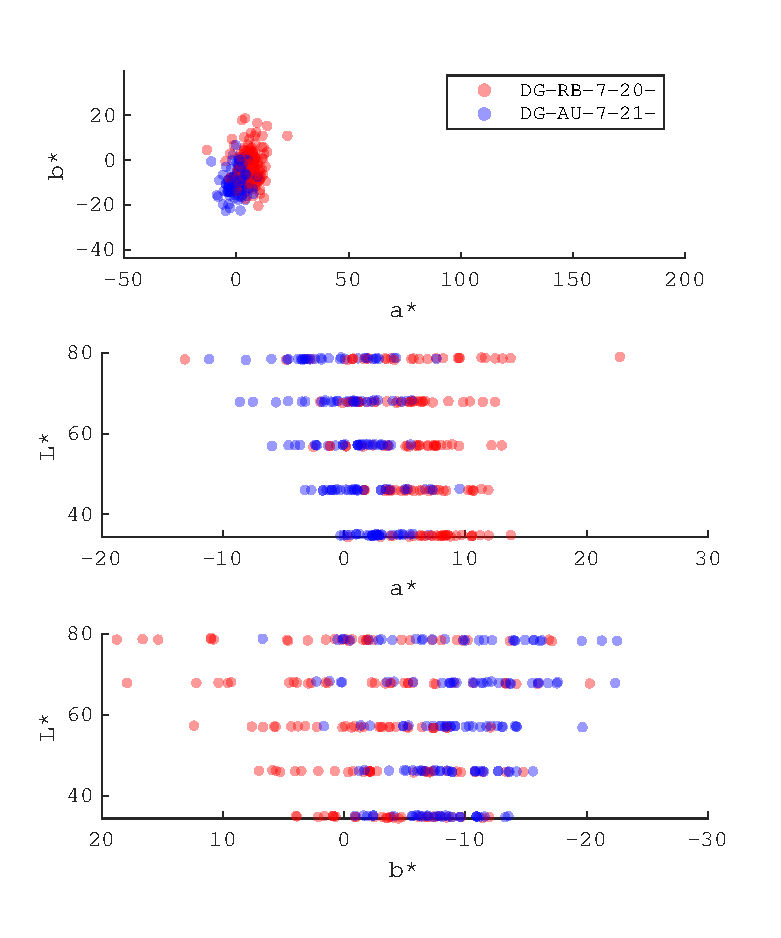
\includegraphics[max width=1.2\textwidth,center]{figs/SmallSphere/DG.pdf}
\caption{Data for observer DG in CIELAB from the 3 different perspectives upon CIELAB. Colour-coding and legend as in Figure \ref{fig:SSsummary}.}
\label{fig:SS_DG}
\end{figure}

\npdecimalsign{.}
\nprounddigits{2}
\begin{table}[htbp]
\begin{tabular}{l|n{5}{2}|n{5}{2}|n{5}{2}|n{5}{2}|n{5}{2}|n{5}{2}} %would be nice to know what the 5,2 does, I just grabbed this off stackoverflow.
 & {Mean L*} & {Mean a*} & {Mean b*} & {SD L*} & {SD a*} & {SD b*} \\\hline
DG-AU-7-21- & 56.9524882586103 & 0.675133479973983 & -8.95624509045388 & 15.4782221350432 & 3.37322583046715 & 5.16326018479416 \\
DG-RB-7-20- & 56.8352131214145 & 5.86729467342570 & -2.25622136024552 & 15.5393088290294 & 4.30521317526720 & 7.16328133963527 \\
HC-AU-7-21- & 56.9830459740028 & 0.402247732505120 & -11.9578449508451 & 15.5435035776612 & 8.21945088677043 & 12.5222120194318 \\
HC-AU-10-18 & 56.8971211534733 & -2.24456088531061 & -7.16804458897986 & 15.4181956290139 & 10.8454390151009 & 13.6183962570021 \\
HC-RB-7-20- & 57.3862272800228 & 6.73813216259034 & -12.2093568428256 & 15.4736742570885 & 8.67549550271706 & 11.2009394810601 \\
HC-RB-10-19 & 57.0530929390755 & 3.71380245778532 & -2.54846686713661 & 15.3993164407270 & 8.83695463046939 & 10.7859514864323 \\
LW-RB-7-21- & 57.5105253571841 & 3.39002741980479 & 20.4596724371518 & 15.4739311348141 & 10.0877780537142 & 12.4311707631679 \\
LW-RB-10-12 & 57.0631633891158 & 44.9631108112767 & 10.4401095935665 & 14.9296460299345 & 13.4200150486452 & 11.1293401028562 \\
LW-AU-7-20- & 57.5360205801163 & 3.60347851990418 & 17.5738374140498 & 15.4155618340430 & 8.35162097424319 & 10.7933314652044 \\
LW-AU-10-11 & 56.6233765384295 & 43.2106748934748 & 13.5352420755118 & 14.8549410119713 & 14.9631458587677 & 10.6922382005586
\end{tabular}
\caption {Summary of Small Sphere data.}
\label{tab:SS}
\end{table}
\npnoround

\begin{figure}[htbp]
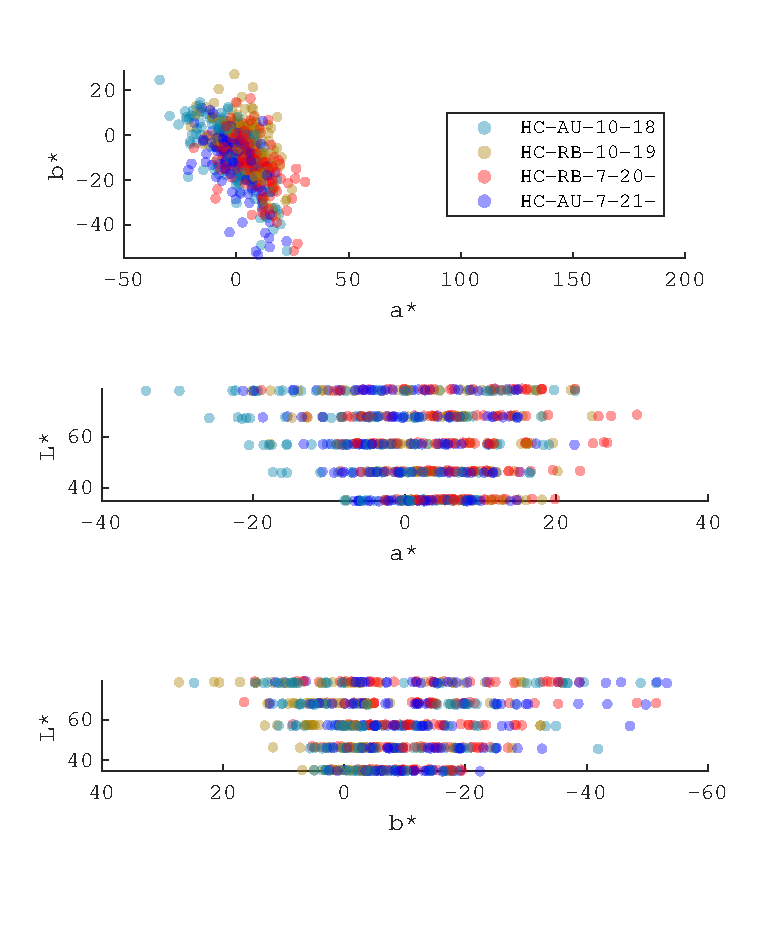
\includegraphics[max width=1.2\textwidth,center]{figs/SmallSphere/HC.pdf}
\caption{As per Figure \ref{fig:SS_DG} but for the data of observer HC.}
\label{fig:SS_HC}
\end{figure}

\begin{figure}[htbp]
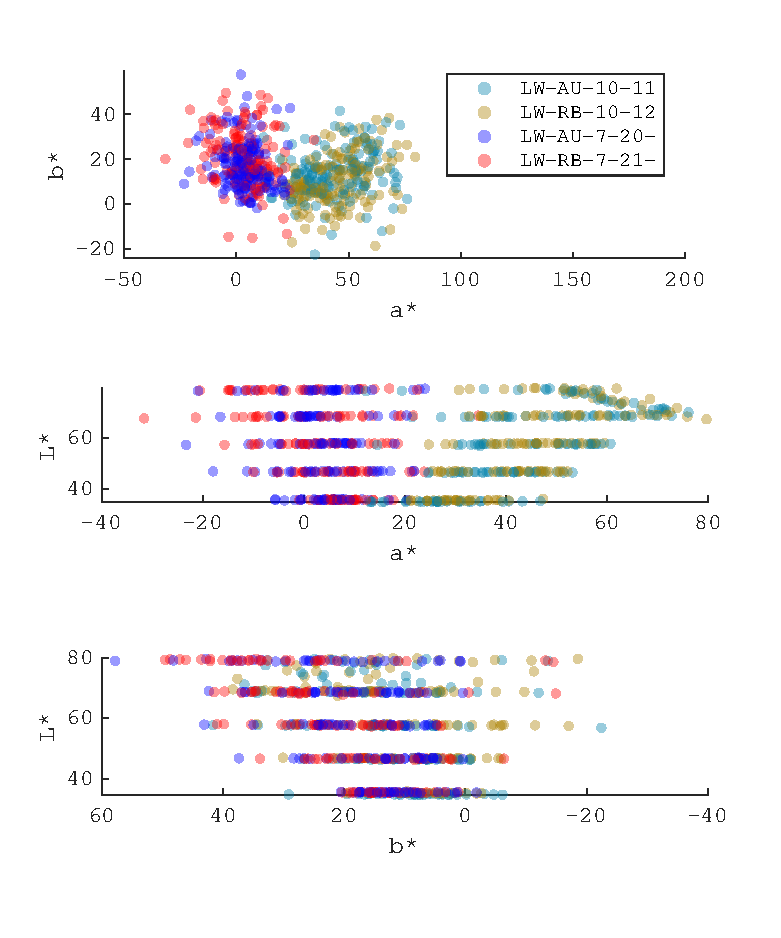
\includegraphics[max width=1.2\textwidth,center]{figs/SmallSphere/LW.pdf}
\caption{As per Figure \ref{fig:SS_DG} but for the data of observer LW.}
\label{fig:SS_LW}
\end{figure} 

All combinations of sets of data were submitted to a two-dimensional two-sample Kolmogorov-Smirnov test\footnote{Using the function available from \url{https://uk.mathworks.com/matlabcentral/fileexchange/38617-kstest_2s_2d-x1-x2-alpha}.}. There was a statistical difference for all combinations ($\alpha$ = 0.05) except LW-AU-7-20- v. LW-RB-7-21-, and LW-AU-10-11 v. LW-RB-10-12. With Bonferroni correction to account for multiple tests ($\alpha$ = 0.05/45 = 0.0011), HC-AU-10-18 v. HC-AU-7-21- additionally fell above the $\alpha$ threshold.

\subsection{Secondary Data}

Data describing the characterisations of hardware follow. Figures \ref{fig:SSLEDs} and \ref{fig:SSLEDs2} show the chromaticities of the adapting surrounds as recorded during each session. 
%
\begin{figure}[htbp]
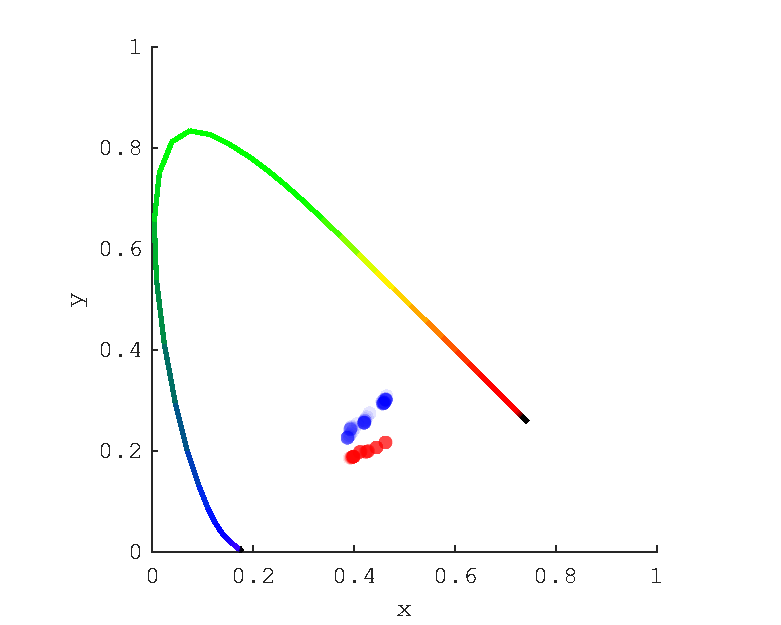
\includegraphics[max width=0.9\textwidth,center]{figs/SmallSphere/OOwide.pdf}
\caption{The \gls{CIE} 1931 chromaticities of the adapting field as measured during data collection, with the spectral locus for context. See figure \ref{fig:SSLEDs2} for further detail.}
\label{fig:SSLEDs}
\end{figure}
%
\begin{figure}[htbp]
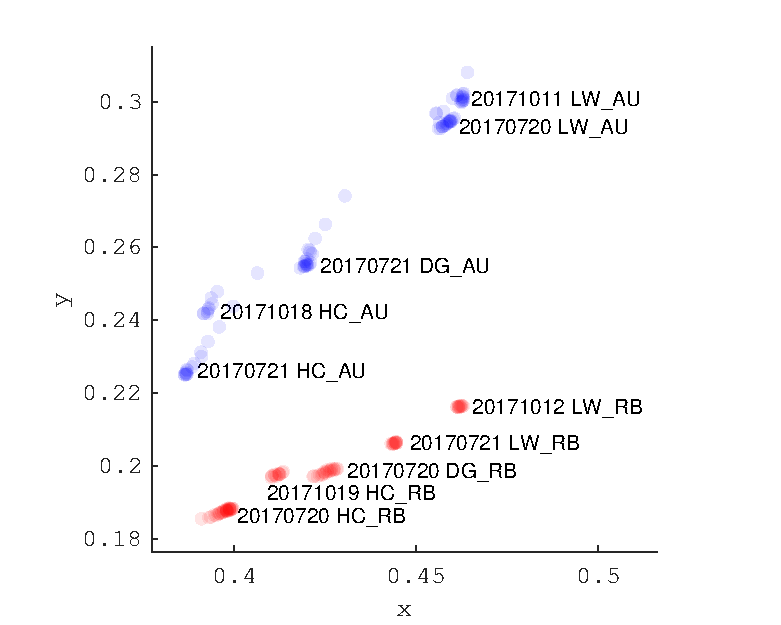
\includegraphics[max width=0.9\textwidth,center]{figs/SmallSphere/OO.pdf}
\caption{As per Figure \ref{fig:SSLEDs} but with different scaling and labels.}
\label{fig:SSLEDs2}
\end{figure}
%
Figure \ref{fig:SSgamut} shows the recorded gamut and white points of the display measured before or after each session. 
%
\begin{figure}[htbp]
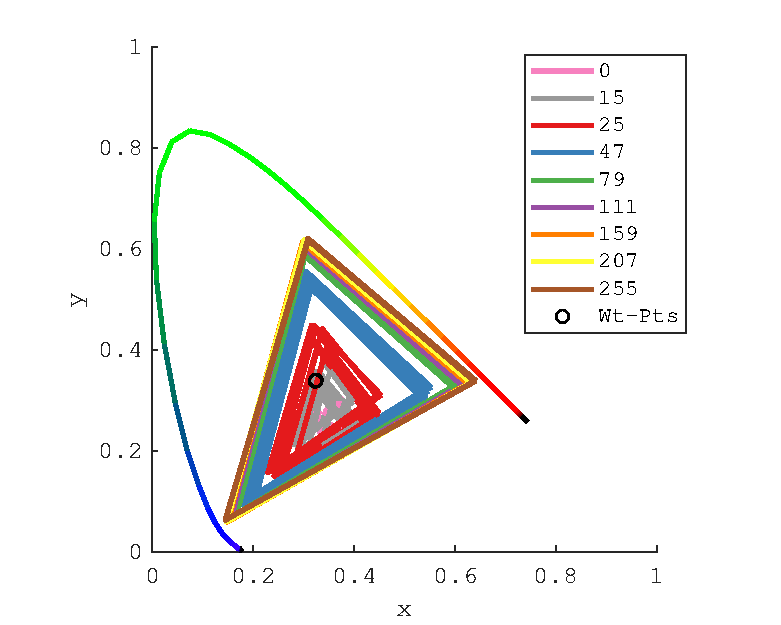
\includegraphics[max width=0.9\textwidth,center]{figs/SmallSphere/SSgamut.pdf}
\caption{The display gamut at multiple pixel output levels, and white points, for all sessions.}
\label{fig:SSgamut}
\end{figure}
%
Figure \ref{fig:SScal2} shows representative results from one of the secondary characterisation sessions.
%
\begin{figure}[htbp]
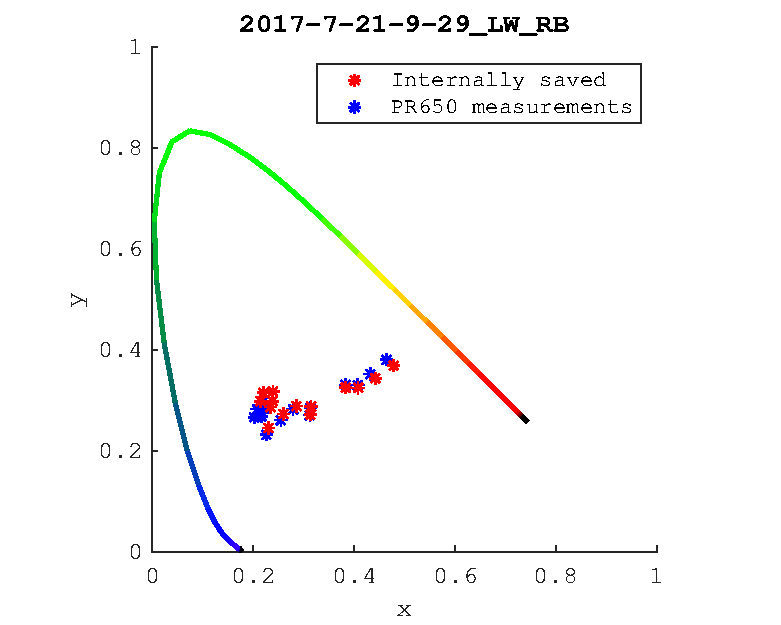
\includegraphics[max width=0.9\textwidth,center]{figs/SmallSphere/SSseccal.pdf}
\caption{Representative results from a single secondary characterisation session.}
\label{fig:SScal2}
\end{figure}

%\clearpage

\section{Discussion}

There were statistically significant differences between the achromatic settings across almost all conditions (exclusions previously noted), including nominal repeat conditions. Most of these differences were relatively minor in magnitude, and within the range of what might reasonably be expected from various inherent sources of error and/or noise.

For one observer (LW), there were not significant differences between the different conditions, but there was a large magnitude difference between the repeat conditions (See Figure \ref{fig:SSsummary} or \ref{fig:SS_LW}). To be clear - with a single day separating inter-condition trials, this observer exhibited no difference between conditions, but after roughly three months, when returning to do a second pair of trials (again with a single day separating) the results were strikingly different. This is particularly unusual considering how well matched the inter-condition responses are; if it were just the case that this particular observer was particularly unreliable in their selections (and their data does exhibit generally quite high standard deviations, see Table \ref{tab:SS}) then I posit that they would be as unlikely to be able to repeat their selections after a break of a day as they would be after a break of three months.

The differences cannot readily be explained by hardware issues; variation in the surround illumination and screen output are minimal between sessions. Further, the same level of variations were present for both observer LW and observer HC.

Regarding Figure \ref{fig:SSLEDs2}, which shows the chromaticities of the peripheral illumination, it can be seen that there was some variation between repeated conditions, and also a small amount of variation within each session. The variation across sessions is likely due to physical disturbance of the equipment (either the measurement device or the illumination source) and is of a relatively minor magnitude. The variation within session seems to be systematic, perhaps relating to warm-up time of the illumination source, with the chromaticity being quite variable for the first few minutes of several trials before gaining stability.

Figures \ref{fig:SSgamut} and \ref{fig:SScal2} show the results of the primary and secondary characterisation protocols respectively. Figure \ref{fig:SSgamut} summarises all the collected data, showing that at very low pixel values there is a moderate level of variability, which seems to correspond to the sphere illumination, suggesting that some illumination from the sphere does reach the screen. Figure \ref{fig:SSgamut} also shows the recorded white point of the screen for each characterisation, but these points stack fairly precisely atop one another. Figure \ref{fig:SScal2} shows a representative set of results from the secondary characterisation protocol (for observer `LW', under red-blue adapting illumination, initial trial - 7/21). It can be seen that there is some distortion between the values as recorded (following calibration) and the measured screen output. There are several potential sources for this error; the calibration routine (for the calibration we rely on tristimulus values computed directly by the \gls{PR650}, whereas for the measurements we record a spectrum and then compute our own tristimulus values), the experimental code (there are a large number of colour-space conversions in the experimental code, it is possible that one has a minor error), amongst others. Importantly, the distortion seems to be systematic (a slight rotation of points roughly around the white point) and of regular magnitude across sessions.

This suggests that there must be some other cause for the difference between LW's first set of data and the repeats. Since it is not the focus of this investigation I shall not dwell upon this point, but I shall suggest two possible causes which have presented themselves. 

The first - although relatively clear instructions were given to observers, it is possible that observer LW chose a distinct interpretation of instructions for the second set of measurements. Specifically, it is possible that the observer switched between making a `hue / saturation / brightness match' to making a `surface-colour' match. It does seem to be the case that for the second pair of datasets, the chosen white points are considerably closer to the chromaticity that a neutral surface would possess, so much so that some responses from this observer hit the display gamut (this is what causes the degradation of data visible in the top right hand corner of the middle plot of Figure \ref{fig:SS_LW}).

The second, though I am aware that this sounds rather fanciful, is that this result could represent a genuine shift in the perception of the observer between sessions. Though it seems unlikely that such a drastic change could result from such, in the absence of other options I feel it is worth considering. There is evidence to suggest that an observer's white point may change seasonally \cite{welbourne_human_2015}, as an effect of changing chromatic distributions of one's surroundings. Three months between sessions seems like a reasonable time-frame within which to witness such a change, particularly when the difference is between July and October (Summer to Autumn), where it is most likely that there would have been a considerable difference in the lushness of vegetation.

One argument against this line of reasoning is that observer HC did not exhibit a similar shift over the same time-frame. It is quite possible however, that one observer had a greater level of exposure to natural (and thus chromatically changing) conditions during this time.

The data of observer HC by comparison shows a high level of regularity. For each session there is a regular orientation of variance (see Figure \ref{fig:SSsummary}), and there is little variation either between conditions or between repeats. What difference there is, could tentatively be considered as systematic - for both the initial and repeat conditions, the RB condition receives responses that are offset to higher a* values compared to the AU condition. Both repeated trials have higher b* means than the initial data-sets, but this change seems to be in line with magnitude and direction of change between the chromaticities of the adapting fields between conditions (see Figure \ref{fig:SSLEDs2}, where the for the second set of recordings the chromaticities have shifted upwards and rightwards in \gls{CIE} 1931 chromaticity space - roughly towards yellow).

The data of observer DG (the author's data) exhibits a lower level of variance (probably due to increased level of familiarity with the test) and exhibits an inter-condition difference of similar magnitude and direction to that for observer HC.

\subsection{Limitations}

One key limitation in this study was that there was no prior prediction of the direction, nor magnitude, of the difference that we expected to see as the effect of changing the melanopic activation. This stems from the fact that though several researchers have sought to examine whether there is a link between melanopsin and colour constancy, none have proposed a clear theory for how or why such involvement might exist.

With the benefit of such a framework we would be much better placed to assess the results of an experiment such as this. As it is, we see minor (but statistically significant) differences between conditions, but struggle to distil signal from noise. As we saw in the Large Sphere experiment, it is very difficult to fully control conditions such that a valuable repeated condition can be performed; all of the dimensions over which a repeat could be performed (time, observer, L*) seem to have meaningful but complex effects!

If there was a model which predicted a specific difference with a predicted orientation and magnitude, it may be possible to use alternative analysis methods which would provide greater clarity. Further, it may be possible to design experiments to more robustly test a more specific hypothesis. Chapter \ref{chap:Melcomp} aims to fill this gap in our understanding.

The other key limitation, which applies equally to this experiment and the Large Sphere Experiment, is that there is an implicit assumption that foveal adaptation is affected by peripheral stimulation. Though this is implicit in all \glspl{CAT} (with only a single transformation applied across an image), it is not clear whether there is a physiological mechanism by which a single transformation could be applied across the entire retina. Indeed we know, from simple experience with after-images, that adaptation to a small area of the retina is certainly possible. It remains unclear what the level of adaptational cross-talk across the retina is. To minimise the impact of this issue, and to increase our understanding of this process, it is recommended that further experiments of this type employ a modified design such that both the periphery and fovea (and further divisions) can be used as both adapting field and test field. Further proposed modifications will be discussed in the final chapter of this thesis.
